The name ATLAS is short for \textit{A Toroidal LHC Apparatus}. It is a multi-purpose particle detector which is designed primarily to detect and measure particles coming out of proton-proton collisions. The detector is located 100 meters underground at the LHC point one so that it is shielded from cosmic rays and weighs about 7000 tons. The ATLAS detector has a forward-backward symmetric cylindrical geometry with radius of 25 meters and length 44 meters. Over three thousand collaborators work at the ATLAS experiment. By design and for cross validation purpose, the ATLAS detector is very similar in regard of its functionality to its counterpart the CMS (Compact Muon Solenoid) detector at LHC point five. 

The collaboration uses a right-handed coordinate system as the convention. The beam pipe which penetrates through the detector is the $z$-axis of the coordinate system, while the origin of which is the beam interaction point (IP) also the center of the detector. The $x$-axis points from the origin of the detector towards the LHC ring center while $y$ axis points upward to the ground. Cylindrical coordinate is used in addition to the Cartesian coordinate described above. The $x-y$ plane parameterized by ($r,\phi$) where $r$ is the radius inside the plane and $\phi$ is the azimuthal angle around the beam. A polar angle $\theta$ is also defined with respect to the beam. The particle pseudorapidity defined as $\eta = -\ln \tan(\theta/2)$ is more commonly used than the polar angle as the difference between two massless particles' pseudorapidity is Lorentz invariant. The measure in the angular plane is defined as $\Delta R = \sqrt{\Delta \phi^2+\Delta \eta^2}$.

The ATLAS detector has approximately $4\pi$ coverage in solid angle. It contains many sub-systems as shown in Fig.\ref{fig:detector-atlas} which are used to measure different properties of the particles as well as distinguish different types of them. The major sub-components are the inner tracking detector, electromagnetic and hadronic calorimeters, and a muon spectrometer. There is also a dedicated data acquisition system to read out, filter and save the massive amount of data collected by these systems. The inner-most part of the detector is the inner detector,more details to be found in Sec.\ref{sec:detector-id}, primarily used to measure the charged-particle trajectories. A superconducting solenoid provides 2T magnetic field pointing in the $z$ direction can bend the charged-particles which will leave energy deposits on the layers of the inner detector, first few of which are silicon pixel layers followed by semiconductor microstrips (SCT) and then a transition radiation tracker (TRT). Most of the particles produced from the collisions end their journey in the calorimeter system, see Sec.\ref{sec:detector-calo}. The combination of electromagnetic lead/liquid-argon (LAr) calorimeter and the hadronic calorimeter built with steel/scintillator tiles measures the energies of particles. Only neutrinos and muons typically go beyond the calorimeters. Neutrinos hardly interact with materials and escape the detector while muons then enters the muon spectrometer with superconducting toroids providing 4T magentic field as will be described in Sec.\ref{sec:detector-mu}. The data coming out of the detector goes through a trigger system (Sec.\ref{sec:detector-trigger}) in order not to swap the disk. First level of filtering is done with level one trigger (L1) implemented in hardware. Another level of software trigger then accepts events at a even smaller rate. 


\begin{figure}[htpb!]
\begin{center}
  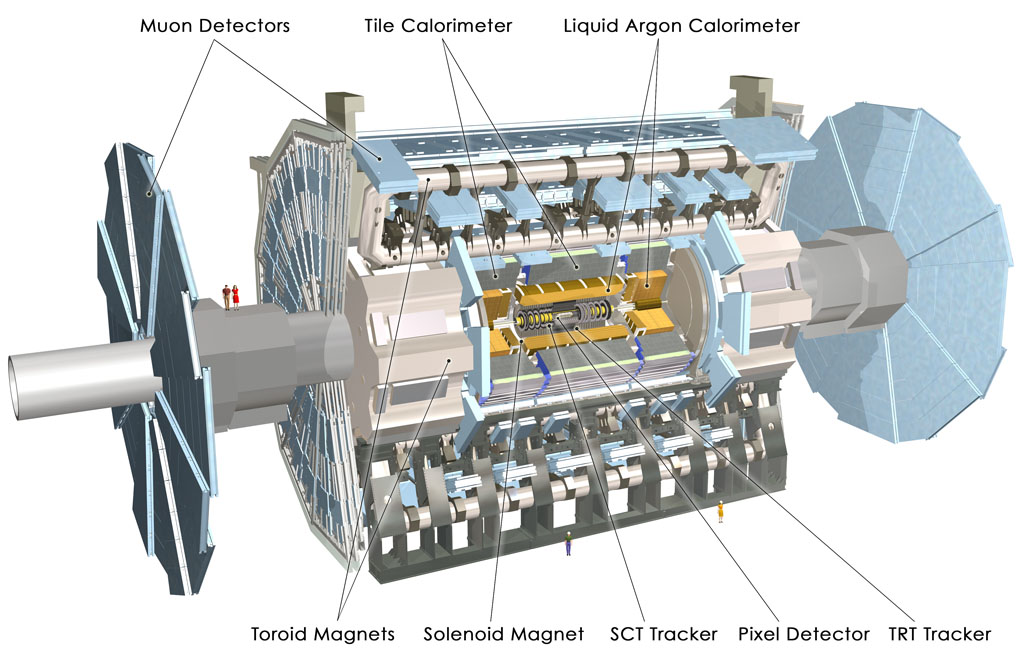
\includegraphics[width=0.85\linewidth]{figures/detector/ATLAS_Silver_White_MK}
\caption{View of the ATLAS detector and its sub-systems}
\label{fig:detector-atlas}
\end{center}
\end{figure}


